\documentclass{beamer}
\usetheme[pageofpages=of,% String used between the current page and the
                         % total page count.
          bullet=circle,% Use circles instead of squares for bullets.
          titleline=true,% Show a line below the frame title.
          alternativetitlepage=true,% Use the fancy title page.
       %   titlepagelogo=logo-polito,% Logo for the first page.
       %   watermark=watermark-polito,% Watermark used in every page.
       %   watermarkheight=100px,% Height of the watermark.
       %   watermarkheightmult=4,% The watermark image is 4 times bigger
                                % than watermarkheight.
          ]{Torino}

\setbeamertemplate{footline}{
  \begin{beamercolorbox}[wd=\paperwidth,ht=1ex,dp=1ex]{footline}
    \vspace{5pt} \hspace{1em} \insertframenumber/\inserttotalframenumber
  \end{beamercolorbox}
}

\author{Brendon J. Brewer}
\title{STATS 331 -- Introduction to Bayesian Statistics}
\institute{The University of Auckland}
\date{}


\linespread{1.3}
\usepackage{minted}
\usepackage[utf8]{inputenc}
\usepackage{dsfont}
\newcommand{\given}{\,|\,}
\newcommand{\balpha}{\boldsymbol{\alpha}}
\newcommand{\bmu}{\boldsymbol{\mu}}


\begin{document}

\frame{\titlepage}

\begin{frame}
\begin{center}
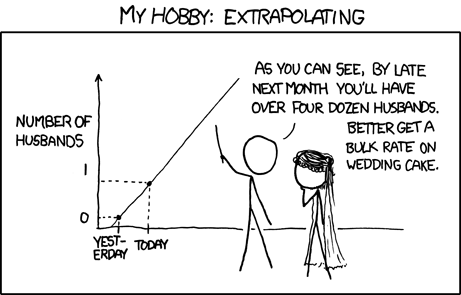
\includegraphics[width=0.6\textwidth]{images/extrapolating.png}

Credit: www.xkcd.com
\end{center}

\end{frame}


\begin{frame}
\Large

\begin{center}
Chi-Squared Test\footnote{Is not a test, and does not involve chi squared.}
\end{center}
\end{frame}


\begin{frame}
\frametitle{Motivating Example}

\begin{center}
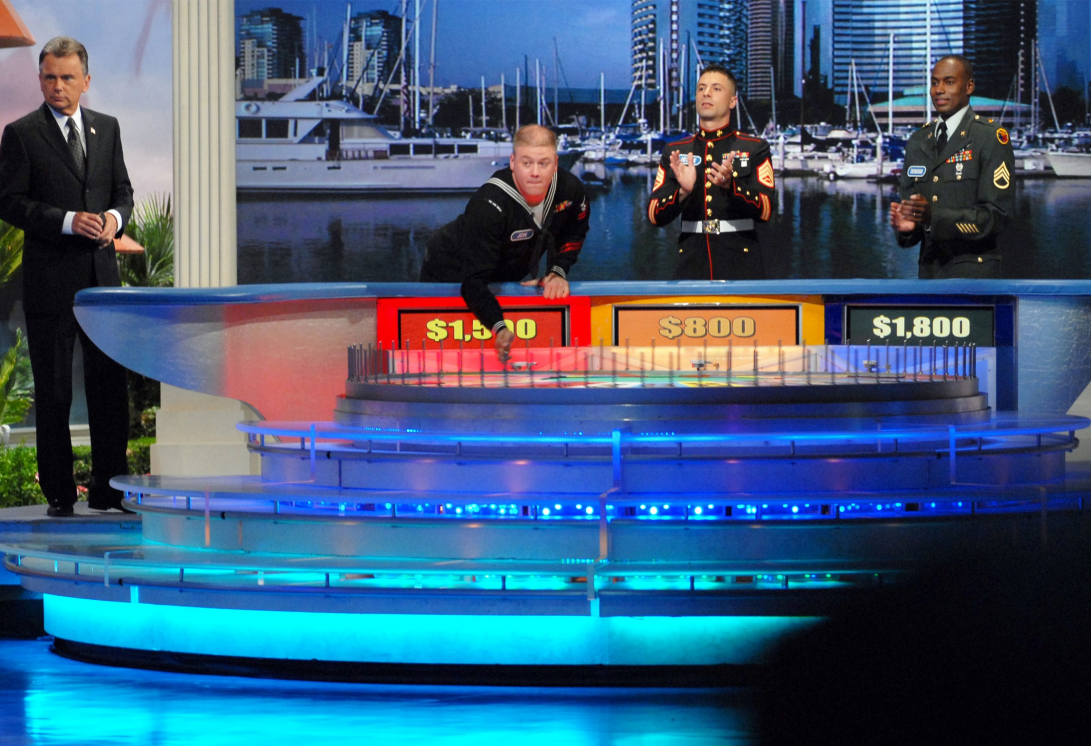
\includegraphics[width=0.6\textwidth]{images/wheel_of_fortune.png}

Source: Wikimedia Commons
\end{center}

\end{frame}


\begin{frame}
\frametitle{The Data}
The outcomes of $N=30$ Wheel of Fortune episodes:

\begin{center}
\begin{tabular}{|c|ccc|}
\hline
Position & 1 & 2 & 3 \\
\hline
Number of Wins $x$ & 8 & 9 & 13 \\
\hline 
\end{tabular}
\end{center}

\end{frame}

\begin{frame}
\frametitle{The Question}
We might wonder whether the following hypothesis is true:\\[0.5em]\pause

$H_0$: There is a 1/3 probability for each position to win each episode.

\end{frame}

\begin{frame}[fragile]
\frametitle{Classical Chi-Squared Test}
The classical `chi-squared test' is designed for this situation.
The test statistic is based on the difference between the observed counts
(8, 9, 13) and the expected counts under $H_0$ (10, 10, 10).
\pause
\begin{minted}{r}
> chisq.test(c(8, 9, 13))

	Chi-squared test for given probabilities

data:  c(8, 9, 13)
X-squared = 1.4, df = 2, p-value = 0.4966
\end{minted}

\end{frame}

\begin{frame}[fragile]
\frametitle{Classical Chi-Squared Test}
The main {\bf advantage} of the classical chi-squared test is that it is very
easy to carry out because it is already implemented in R.\\[0.5em]\pause

The main {\bf disadvantages} are:\pause
\begin{itemize}
\item It returns a p-value, not a posterior probability, and is subject to the
usual objections.\pause
\item It is based on an approximation that assumes that the number of counts
in each bin is high. Typically $\geq 5$ is preferred.
\end{itemize}

\end{frame}

\end{document}

